\section{lg\-Int\-Tag\-Arg Class Reference}
\label{classlgIntTagArg}\index{lgIntTagArg@{lgIntTagArg}}
integer tag argument  


{\tt \#include $<$lgtagarg.h$>$}

Inheritance diagram for lg\-Int\-Tag\-Arg::\begin{figure}[H]
\begin{center}
\leavevmode
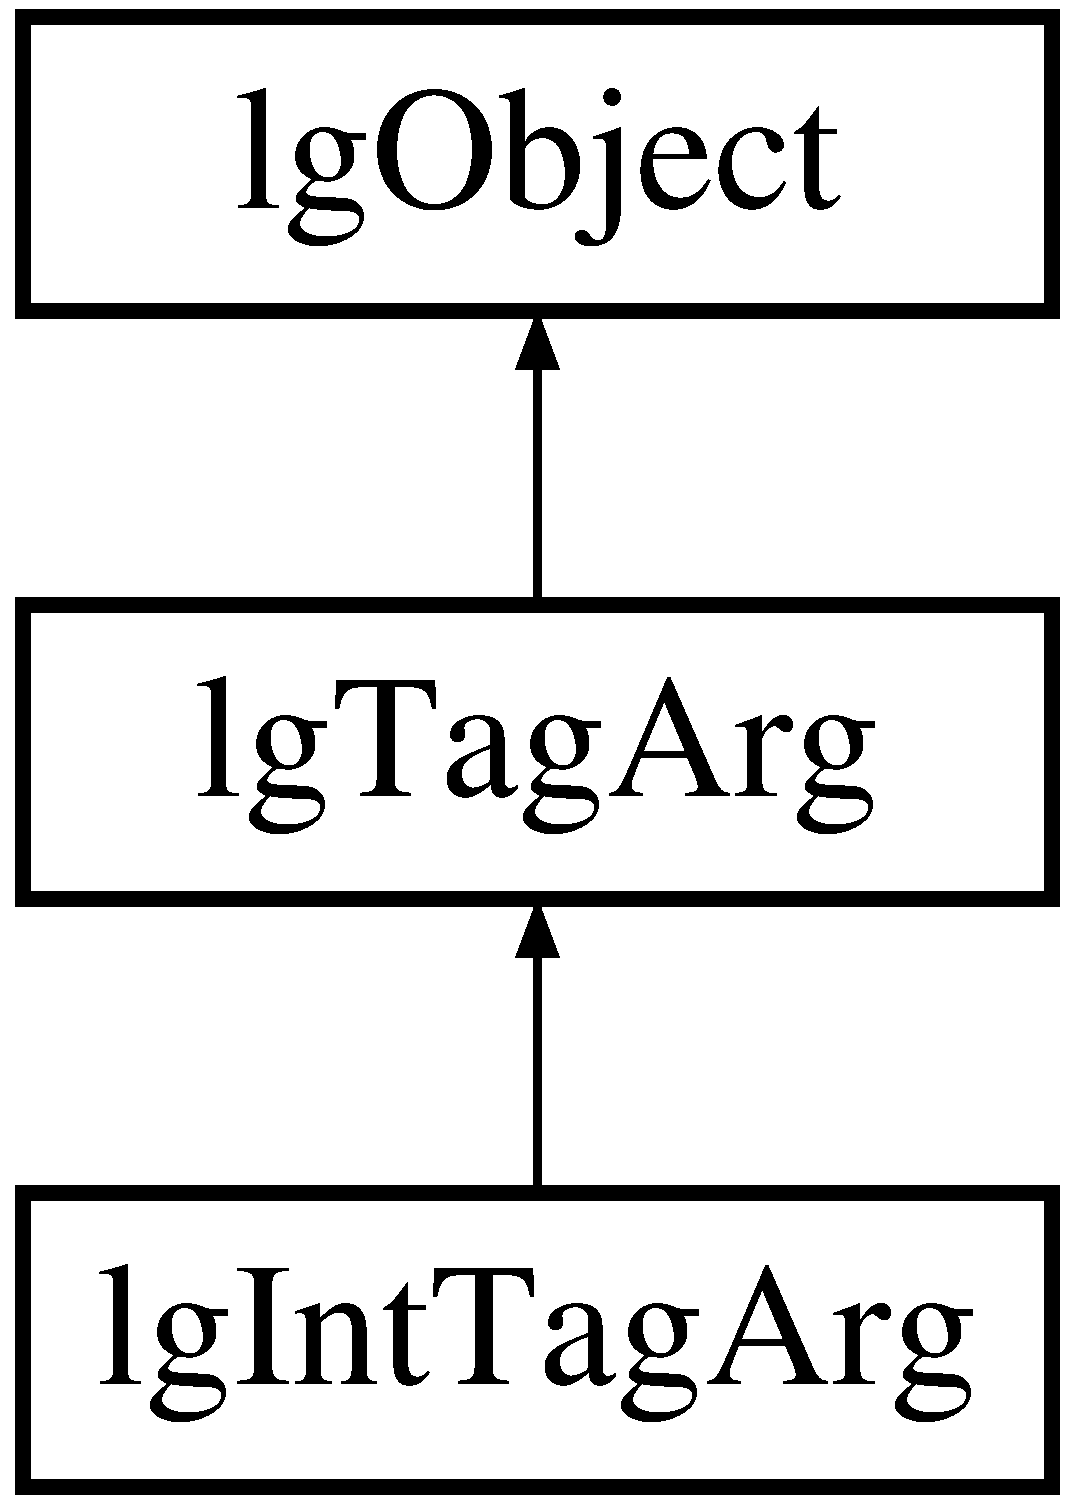
\includegraphics[height=3cm]{classlgIntTagArg}
\end{center}
\end{figure}
\subsection*{Public Member Functions}
\begin{CompactItemize}
\item 
virtual string {\bf to\-String} ({\bf lg\-Voice} $\ast$seq=NULL)
\item 
{\bf lg\-Int\-Tag\-Arg} (const char $\ast$na, int v, const char $\ast$unit=\char`\"{}\char`\"{})
\item 
virtual int {\bf val\-Int} (void)
\item 
virtual double {\bf val\-Float} (void)
\item 
virtual string {\bf val\-Str} (void)
\item 
virtual void {\bf set\-Val\-Int} (int val)
\end{CompactItemize}
\subsection*{Private Attributes}
\begin{CompactItemize}
\item 
int {\bf val\-I}
\end{CompactItemize}


\subsection{Detailed Description}
integer tag argument 



\subsection{Constructor \& Destructor Documentation}
\index{lgIntTagArg@{lg\-Int\-Tag\-Arg}!lgIntTagArg@{lgIntTagArg}}
\index{lgIntTagArg@{lgIntTagArg}!lgIntTagArg@{lg\-Int\-Tag\-Arg}}
\subsubsection{\setlength{\rightskip}{0pt plus 5cm}lg\-Int\-Tag\-Arg::lg\-Int\-Tag\-Arg (const char $\ast$ {\em na}, int {\em v}, const char $\ast$ {\em unit} = \char`\"{}\char`\"{})}\label{classlgIntTagArg_a1}


\begin{Desc}
\item[Parameters: ]\par
\begin{description}
\item[{\em 
na}]argument name, might be \char`\"{}\char`\"{} \item[{\em 
v}]argument value \end{description}
\end{Desc}


\subsection{Member Function Documentation}
\index{lgIntTagArg@{lg\-Int\-Tag\-Arg}!setValInt@{setValInt}}
\index{setValInt@{setValInt}!lgIntTagArg@{lg\-Int\-Tag\-Arg}}
\subsubsection{\setlength{\rightskip}{0pt plus 5cm}virtual void lg\-Int\-Tag\-Arg::set\-Val\-Int (int {\em val})\hspace{0.3cm}{\tt  [inline, virtual]}}\label{classlgIntTagArg_a5}


\index{lgIntTagArg@{lg\-Int\-Tag\-Arg}!toString@{toString}}
\index{toString@{toString}!lgIntTagArg@{lg\-Int\-Tag\-Arg}}
\subsubsection{\setlength{\rightskip}{0pt plus 5cm}string lg\-Int\-Tag\-Arg::to\-String ({\bf lg\-Voice} $\ast$ {\em v} = NULL)\hspace{0.3cm}{\tt  [virtual]}}\label{classlgIntTagArg_a0}


get GUIDO string should be redefined in all derived classes 

Reimplemented from {\bf lg\-Tag\-Arg} {\rm (p.\,\pageref{classlgTagArg_a0})}.\index{lgIntTagArg@{lg\-Int\-Tag\-Arg}!valFloat@{valFloat}}
\index{valFloat@{valFloat}!lgIntTagArg@{lg\-Int\-Tag\-Arg}}
\subsubsection{\setlength{\rightskip}{0pt plus 5cm}virtual double lg\-Int\-Tag\-Arg::val\-Float (void)\hspace{0.3cm}{\tt  [inline, virtual]}}\label{classlgIntTagArg_a3}




Reimplemented from {\bf lg\-Tag\-Arg} {\rm (p.\,\pageref{classlgTagArg_a5})}.\index{lgIntTagArg@{lg\-Int\-Tag\-Arg}!valInt@{valInt}}
\index{valInt@{valInt}!lgIntTagArg@{lg\-Int\-Tag\-Arg}}
\subsubsection{\setlength{\rightskip}{0pt plus 5cm}virtual int lg\-Int\-Tag\-Arg::val\-Int (void)\hspace{0.3cm}{\tt  [inline, virtual]}}\label{classlgIntTagArg_a2}




Reimplemented from {\bf lg\-Tag\-Arg} {\rm (p.\,\pageref{classlgTagArg_a4})}.\index{lgIntTagArg@{lg\-Int\-Tag\-Arg}!valStr@{valStr}}
\index{valStr@{valStr}!lgIntTagArg@{lg\-Int\-Tag\-Arg}}
\subsubsection{\setlength{\rightskip}{0pt plus 5cm}virtual string lg\-Int\-Tag\-Arg::val\-Str (void)\hspace{0.3cm}{\tt  [inline, virtual]}}\label{classlgIntTagArg_a4}




Reimplemented from {\bf lg\-Tag\-Arg} {\rm (p.\,\pageref{classlgTagArg_a3})}.

\subsection{Member Data Documentation}
\index{lgIntTagArg@{lg\-Int\-Tag\-Arg}!valI@{valI}}
\index{valI@{valI}!lgIntTagArg@{lg\-Int\-Tag\-Arg}}
\subsubsection{\setlength{\rightskip}{0pt plus 5cm}int {\bf lg\-Int\-Tag\-Arg::val\-I}\hspace{0.3cm}{\tt  [private]}}\label{classlgIntTagArg_r0}




The documentation for this class was generated from the following files:\begin{CompactItemize}
\item 
{\bf lgtagarg.h}\item 
{\bf lgtagarg.cpp}\end{CompactItemize}
